\documentclass{article}

\title{LO12 - TP01}
\author{Maxime Huyghe}

\usepackage[french]{babel}
\usepackage{minted}
\usepackage{graphicx}

\begin{document}

\maketitle

\section*{Exercice 3}

Code testé :
\begin{minted}{prolog}
inc([X], [Y]) :- Y is X + 1.
inc([X | XRest], [Y | YRest]) :- Y is X + 1, inc(XRest, YRest).
\end{minted}

Requêtes testées et leur premier résultat :
\begin{minted}{prolog}
inc([2], R). R = [3].
inc([], R). false.
inc([1, 2], R). R = [2, 3].
inc([2], [3]). true.
inc([2], [2]). false.
inc([2], [4]). false.
\end{minted}

Arbre de résolution de la requète \mintinline{prolog}{inc([1, 2], R).} :

% \begin{figure}[h]
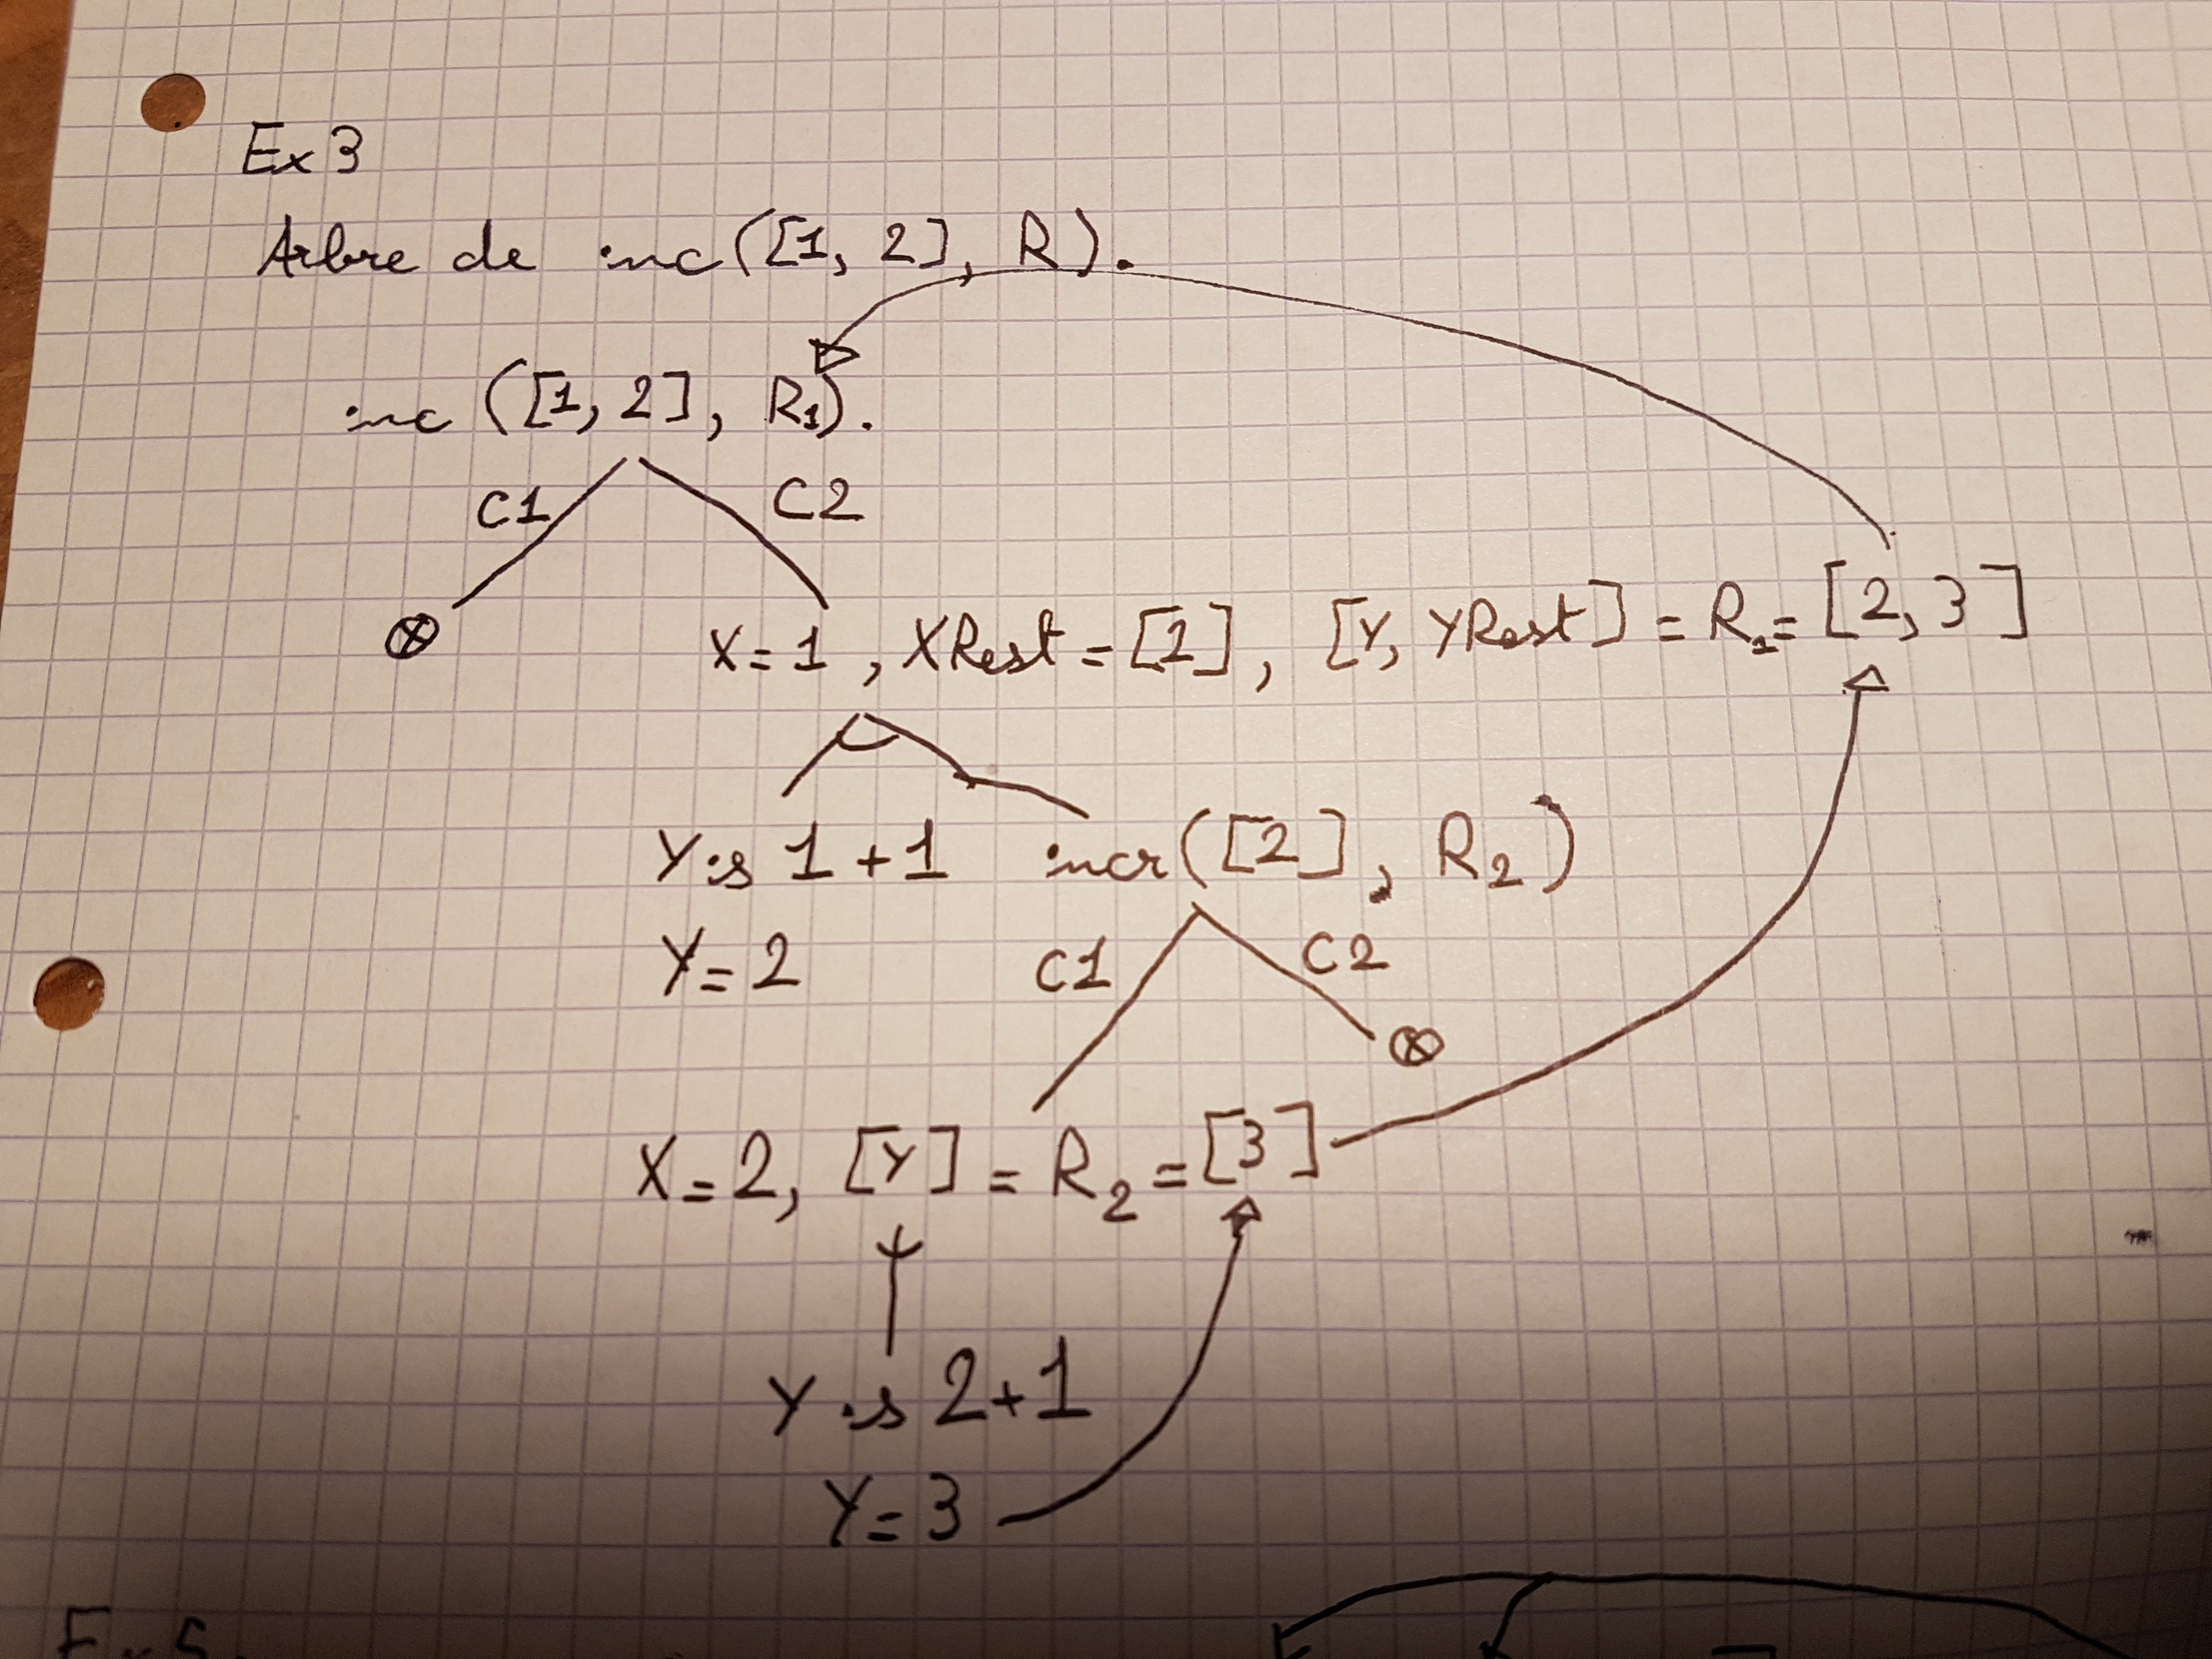
\includegraphics[width=\textwidth]{arbre_ex3}
% \end{figure}

Trace d'exécution de la requète \mintinline{prolog}{inc([1, 2], R).} :
\begin{minted}{prolog}
[trace]  ?- inc([1, 2], R).
   Call: (8) inc([1, 2], _4404) ? creep
   Call: (9) _4636 is 1+1 ? creep
   Exit: (9) 2 is 1+1 ? creep
   Call: (9) inc([2], _4638) ? creep
   Call: (10) _4648 is 2+1 ? creep
   Exit: (10) 3 is 2+1 ? creep
   Exit: (9) inc([2], [3]) ? creep
   Exit: (8) inc([1, 2], [2, 3]) ? creep
R = [2, 3] .
\end{minted}

Il n'y a aucune différence d'exécution entre l'arbre et la trace.

\section*{Exercice 4 - original}

Code testé :
\begin{minted}{prolog}
/*B1*/ ancetre(X,Y):-parent(X,Z), ancetre(Z,Y).
/*B2*/ ancetre(X,Y):-parent(X,Y).
/*B3*/ parent(paul, jacques).
/*B4*/ parent(marie, jacques).
/*B5*/ parent(jacques, lili).
/*B6*/ parent(martine, lili).
\end{minted}

Requête testée :
\begin{minted}{prolog}
ancetre(paul, lili). true.
\end{minted}

Arbre de résolution de la requète \mintinline{prolog}{ancetre(paul, lili).} :
diapo cours

Trace d'exécution de la requète \mintinline{prolog}{ancetre(paul, lili).} :
\begin{minted}{prolog}
?- trace, ancetre(paul, lili).
   Call: (9) ancetre(paul, lili) ? creep
   Call: (10) parent(paul, _732) ? creep
   Exit: (10) parent(paul, jacques) ? creep
   Call: (10) ancetre(jacques, lili) ? creep
   Call: (11) parent(jacques, _732) ? creep
   Exit: (11) parent(jacques, lili) ? creep
   Call: (11) ancetre(lili, lili) ? creep
   Call: (12) parent(lili, _732) ? creep
   Fail: (12) parent(lili, _732) ? creep
   Redo: (11) ancetre(lili, lili) ? creep
   Call: (12) parent(lili, lili) ? creep
   Fail: (12) parent(lili, lili) ? creep
   Fail: (11) ancetre(lili, lili) ? creep
   Redo: (10) ancetre(jacques, lili) ? creep
   Call: (11) parent(jacques, lili) ? creep
   Exit: (11) parent(jacques, lili) ? creep
   Exit: (10) ancetre(jacques, lili) ? creep
   Exit: (9) ancetre(paul, lili) ? creep
true .
\end{minted}

Il n'y a aucune différence d'exécution entre l'arbre et la trace.

\section*{Exercice 4 - variante}

Code testé :
\begin{minted}{prolog}
/*B1*/ ancetre(X,Y):- ancetre(Z,Y), parent(X,Z).
/*B2*/ ancetre(X,Y):-parent(X,Y).
/*B3*/ parent(paul, jacques).
/*B4*/ parent(marie, jacques).
/*B5*/ parent(jacques, lili).
/*B6*/ parent(martine, lili).
\end{minted}

Requête testée :
\begin{minted}{prolog}
ancetre(paul, lili). true.
\end{minted}

Arbre de résolution de la requète \mintinline{prolog}{ancetre(paul, lili).} :
diapo cours

Trace d'exécution de la requète \mintinline{prolog}{ancetre(paul, lili).} :
\begin{minted}{prolog}
[trace]  ?- trace, ancetre(paul, lili).
   Call: (9) ancetre(paul, lili) ? creep
   Call: (10) ancetre(_1240, lili) ? creep
   Call: (11) ancetre(_1240, lili) ? creep
   Call: (12) ancetre(_1240, lili) ? creep
   Call: (13) ancetre(_1240, lili) ? creep
   Call: (14) ancetre(_1240, lili) ? creep
   Call: (15) ancetre(_1240, lili) ? creep
   Call: (16) ancetre(_1240, lili) ? creep
   Call: (17) ancetre(_1240, lili) ? creep
   Call: (18) ancetre(_1240, lili) ? creep
   Call: (19) ancetre(_1240, lili) ? creep
   Call: (20) ancetre(_1240, lili) ? creep
   Call: (21) ancetre(_1240, lili) ? creep
   Call: (22) ancetre(_1240, lili) ? creep
   Call: (23) ancetre(_1240, lili) ? creep
   Call: (24) ancetre(_1240, lili) ? creep
   Call: (25) ancetre(_1240, lili) ? creep
   Call: (26) ancetre(_1240, lili) ? creep
   Call: (27) ancetre(_1240, lili) ? creep
   Call: (28) ancetre(_1240, lili) ? creep
   Call: (29) ancetre(_1240, lili) ? creep
   Call: (30) ancetre(_1240, lili) ? creep
   Call: (31) ancetre(_1240, lili) ? creep
   Call: (32) ancetre(_1240, lili) ? creep
   Call: (33) ancetre(_1240, lili) ? abort
% Execution Aborted
\end{minted}

Prolog entre en récursion infinie de la même façon que l'arbre du cours.

\section*{Exercice 6}

Code testé :
\begin{minted}{prolog}
/* pour simplifier le programme */
contains([X | _], X).
contains([_ | RL], X) :- contains(RL, X).

diff([], _, []).
diff([X | XL], YL, [X | RL]) :- not(contains(YL, X)), diff(XL, YL, RL).
diff([X | XL], YL, RL) :- contains(YL, X), diff(XL, YL, RL).
/* je ne vois pas comment utiliser la coupure */
\end{minted}

Requêtes testées et leur première réponse :
\begin{minted}{prolog}
?- diff([], [], R).
R = [].
?- diff([1, 2], [], R).
R = [1, 2] .
?- diff([1, 2], [3, 4], R).
R = [1, 2] .
?- diff([1, 2], [1, 4], R).
R = [2].
?- diff([1, 2, 5, 46], [1, 3, 5, 6 ], R).
R = [2, 46] .
\end{minted}

Arbre de résolution de la requète \mintinline{prolog}{diff([1, 2], [1], R).} :

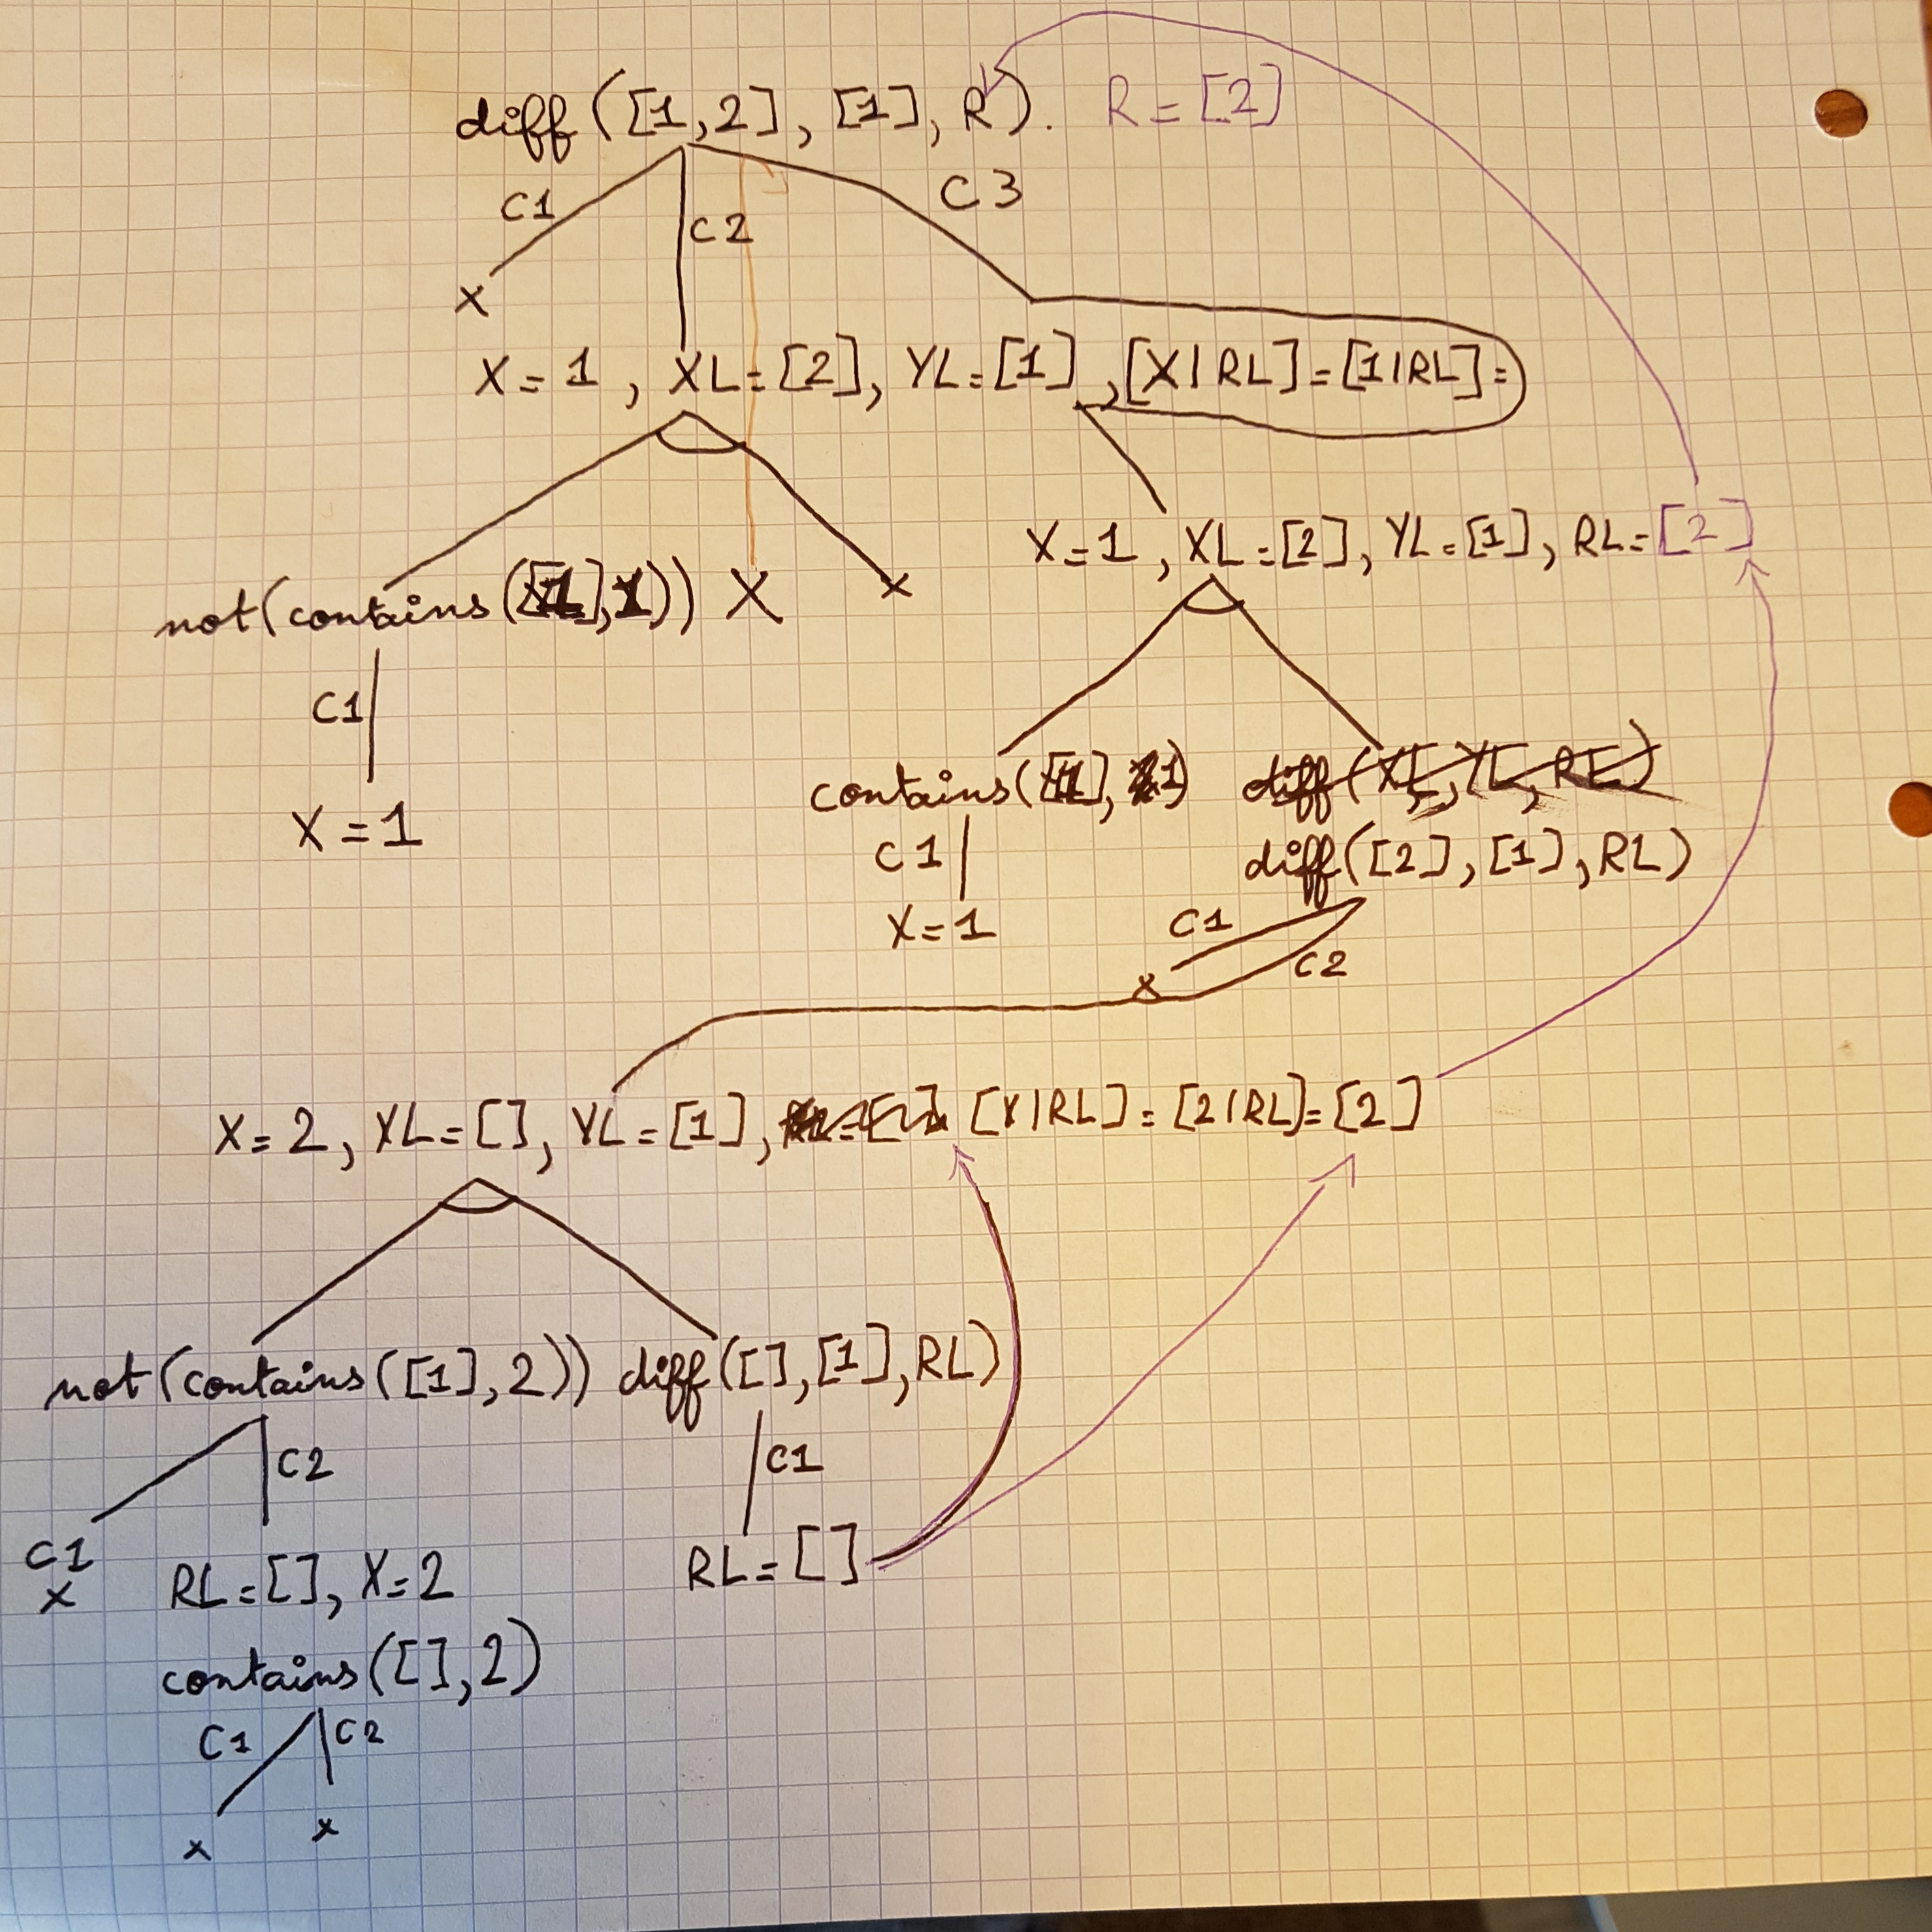
\includegraphics[width=\textwidth]{arbre_ex6}

Trace d'exécution de la requète \mintinline{prolog}{diff([1, 2], [1], R).} :
\begin{minted}{prolog}
[trace]  ?- diff([1, 2], [1], R).
   Call: (10) diff([1, 2], [1], _5222) ? creep
^  Call: (11) not(contains([1], 1)) ? creep
   Call: (12) contains([1], 1) ? creep
   Exit: (12) contains([1], 1) ? creep
^  Fail: (11) not(user:contains([1], 1)) ? creep
   Redo: (10) diff([1, 2], [1], _5222) ? creep
   Call: (11) contains([1], 1) ? creep
   Exit: (11) contains([1], 1) ? creep
   Call: (11) diff([2], [1], _5222) ? creep
^  Call: (12) not(contains([1], 2)) ? creep
   Call: (13) contains([1], 2) ? creep
   Call: (14) contains([], 2) ? creep
   Fail: (14) contains([], 2) ? creep
   Fail: (13) contains([1], 2) ? creep
^  Exit: (12) not(user:contains([1], 2)) ? creep
   Call: (12) diff([], [1], _6004) ? creep
   Exit: (12) diff([], [1], []) ? creep
   Exit: (11) diff([2], [1], [2]) ? creep
   Exit: (10) diff([1, 2], [1], [2]) ? creep
R = [2] .
\end{minted}

L'arbre correspond à la trace.

\end{document}